\documentclass[a4paper,11pt]{article}

\usepackage{amsmath,amssymb,amsfonts}
\usepackage{booktabs}
\usepackage[dvipsnames]{xcolor}
\usepackage[margin=30mm]{geometry}
\usepackage{graphicx}
	\graphicspath{
		{graphics/}
	}
\usepackage{hyperref}
	\hypersetup{
		colorlinks=true,
		linkcolor=blue,
		filecolor=blue,
		urlcolor=blue,
		citecolor=blue
	}
%\usepackage[sort&compress]{natbib}
%	\bibliographystyle{apalike}
\usepackage{soul}
\usepackage{url}


% Damien added packages
\usepackage{listings}
\lstset{language=R,
    basicstyle=\small\ttfamily,
    stringstyle=\color{DarkGreen},
    otherkeywords={0,1,2,3,4,5,6,7,8,9},
    morekeywords={TRUE,FALSE},
    deletekeywords={data,frame,length,as,character},
    keywordstyle=\color{blue},
    commentstyle=\color{DarkGreen},
}
\usepackage{float}
\usepackage{subfig}

\newcommand{\jwj}[1]{{\color{red}{~(jwj: #1)}}}
\newcommand{\yourInitials}[1]{{\color{blue}{~(yourInitials: #1)}}}

\usepackage{titlesec}
\titleformat{\section}{\normalfont\large\bfseries}{}{0pt}{}
\titleformat{\subsection}{\normalfont\large\bfseries}{}{10pt}{}
\titleformat{\subsubsection}{\normalfont\small\bfseries}{}{30pt}{}


%=======================================

%Note: Include constraints that ensure if i=1 is selected, all t's in i=1 must be activated too. If i is on then all t's must be on too.

\title{BOZ780 Assignment 1}
\author{DS de Gouveia \\ 15003079}
\date{\today}

\begin{document}
\maketitle
\tableofcontents
\newpage

\section{Question 1}\label{q1}
\subsection{Question 1 (a) - Stochastic program formulation}

\subsubsection{Assumptions}
\begin{itemize}
	\item If a project is selected all of it's cash flows will be implemented. If two or more projects are selected, their combined cashflow requirement is aggregated and compared to the available cash flow.
	\item The cashflows of each project may change but the NPV will remain the same, that is the NPV is independent on the cashflow. 
\end{itemize}


\subsubsection{Problem formulation}

\begin{tabular}{ll}
$T$ & set of years $T \in (1,2,3)$ \\
$I$ & set of projects $I \in (1,\dots, 10)$ 
\end{tabular}\\

\begin{tabular}{ll}
$a_{t} \triangleq$ & cash in millions of dollars available for investment in year $t$, where  $t \in T$\\
$c_{it} \triangleq$ & cost of project $i$ in millions of dollars for year $t$, where $t \in T, i \in I$\\
$n_{i} \triangleq$ & net present value of project $i$, where  $i \in I$\\
\end{tabular}


\begin{tabular}{lll}
$x_{i} \triangleq$ & 
	$\begin{cases} 
      	1 & \text{project $i$ is selected} \\
      	0 & \text{otherwise} 
	\end{cases}$ & $i \in I, j \in J$
\end{tabular}\\

\setcounter{equation}{0}	

The objective of the investment is to increase profitability. The Net Present Value (NPV) is a means of assessing future profitability whilst accounting for inflation. Thus the objective of the model is to maximise the NPV of all projects whilst adhering to cash flow constraints.

\begin{equation}
	\max z = \sum_{i\in I} x_i n_i
\end{equation}

Subject to

\begin{align}
\label{eq:q1a1}
	\sum_{i\in I} x_i\tilde{c}_{it} \leq a_t && \forall t\in T \\
\label{eq:q1a2}
	x_i \in \{0,1\} && \forall i\in I
\end{align}

Of the two constraints, the first has been identified as an uncertain constraint with random variable $\tilde{c}_{it}$. Equation \ref{eq:q1a1} states that for every year $t$ the total cost of projects $i$ must be less than or equal to the available cashflow $a_t$, noting that $\tilde{c}_{it}$ is a random variable following a uniform distribution.

\newpage

%================================================================

\subsection{Question 1 (b) - Chance constraint scenario approach}
The following question refers to the previously defined formulation in Question \ref{q1}.

\subsubsection{Problem formulation}
The expected value formulation is disregarded and the uncertain constraints are reintroduced.

\begin{equation}
	\max z = \sum_{i\in I} x_i n_i
\end{equation}

Subject to

\begin{align}
	\sum_{i\in I} x_i\tilde{c}_{it} \leq a_t && \forall t\in T \label{q1b7}		\\
	x_i \in \{0,1\} && \forall i\in I
\end{align}

Constraint \ref{q1b7} is applicable for 90\% of the time. To accommodate this requirement, the constraint is expressed as
\begin{equation}
	P(\sum_{i\in I} x_i\tilde{c}_{it} \leq a_t)\geq 0.9
	\label{q1b9}
\end{equation}
where $P$ indicates the probability of this constraint being used. To solve this problem, a set of $N$ constraints must be derived from a random sample of the uniformly distributed variable $\tilde{c}_{it}$ which will convert equation \ref{q1b9} into the following form.
\begin{align}
	P\big{(}F(x,\zeta^v)\leq 0 \big{)} \geq 1 - \alpha && v=1,\dots,N
\end{align}

The scenario approach is implemented as follows.

\begin{align}
	P(\sum_{i\in I} x_i\tilde{c}_{it} \leq a_t)\geq  1-0.1
	\label{q1b11}
\end{align}

From this form we can deduce that $\alpha = 0.1$ and $n= 10$. It is then assumed that a 99\% confidence interval should be applied resulting in a $\delta = 0.01$. The confidence interval ensures that 99\% of the samples will satisfies the constraint 90\% of the time. These values are used to calculate the number of $N$ samples  using the following formula.

\begin{align}
	N=[ 2n\alpha^{-1}\ln(\frac{12}{\alpha}) + 2\alpha^{-1}\ln(\frac{2}{\delta})+2n]
	\label{q1eqN}
\end{align}

The known values are inserted into the formula and $N$ is calculated.

\begin{align}
	N&=[ 2(10)(0.1)^{-1}\ln(\frac{12}{0.1}) + 2(0.01)^{-1}\ln(\frac{2}{0.01})+2(10)]\\
	N& = 1083.465 \approx 1084
\end{align}

The constraint may be reformulated as 

\begin{align}
	\sum_{i\in I} x_ic^{q}_{it} \leq a_t && \forall q\in Q, \forall t \in T
\end{align}

where $|Q| = N = 1084$ is the sample set.

\newpage




%================================================================

\subsection{Question 1 (c) - Credit shortfall}

\subsubsection{Assumptions}
The following question refers to the previously defined formulation in Question \ref{q1}.

\subsubsection{Stochastic problem formulation}
The non-deterministic formulation shall be re-formulated into a recourse programme. Doing so will include a recourse variable in the constraint that captures the deficient cashflow amount which is the difference between $a_t$ and the total cost of the projects. The deficiency is then penalised in the objective function using the 15\% interest rate as a scaler quantity. The following recourse programme extends the formulation in Question \ref{q1}.

%check and see if you can describe the problem 

\vspace{12pt}

\begin{tabular}{ll}
$e_{t} \triangleq$ & compounded interest rate applied in year $t$, where  $t \in T$ for \{1.15,1.32,1.52\}\\
$\delta_{t}^- \triangleq$ & cashflow deficit in millions of dollars for year $t$, where $t \in T$\\
$\delta_{t}^+ \triangleq$ & cashflow surplus in millions of dollars for year $t$, where $t \in T$
\end{tabular}

\vspace{12pt}

The $\delta_{t}^-$ recourse variable captured the cashflow deficient. Including $\delta_{t}^+$ is merely a formality to accommodate the possibility of surplus cashflow, which could only occur if the constraints are tightened (reduced number of projects). For this reason, $\delta_{t}^+$ is not penalised ergo, included in the objective function.

\begin{equation}
	\max z = \sum_{i\in I} x_i n_i - \sum_{t\in T}E_{\tilde{c}_{it}} \big{[}e_t\delta^-_t(\tilde{c}_{it})\big{]}
\end{equation}



Subject to

\begin{align}
	\sum_{i\in I} x_i\tilde{c}_{it} +\delta_{t}^+(\tilde{c}_{it})- \delta^-_t(\tilde{c}_{it})= a_t && \forall t\in T \label{q1b7}	\\
	x_i \in \{0,1\} && \forall i\in I\\
	\delta_{t}^+(\tilde{c}_{it}), \delta^-_t(\tilde{c}_{it})\geq0 && \forall i\in I ,\forall t\in T
\end{align}

\subsubsection{Deterministic problem formulation}
To formulate the stochastic problem into a deterministic equivalent, discrete realisations of the random variable must be created. 

\begin{equation}
	\tilde{c}_{it} \approx \big{\{}(p_1^{r_1},y_1^{r_1,r_2})\big{\}}_{r_1\in R_1}
\end{equation}

where $p_1^{r_1}$ is the probability of impact $y_1^{r_1}$ occurring for realisation $r_1 \in R_1$ where $R_1$ is the set of bins chosen. In this instance, five bins have been selected. Using the \texttt{R} code snippet \ref{code:q1c} the probability and impact for each bin are calculated and results are summarised in Table~\ref{tab:q1cT1}. For each project $i$ the same impact is applicable as they are derived from the same random variable.

The deterministic realisations of the random variable are then included in the model. For each realisation a constraint is added to ensure that under those condition the model remains feasible. The probability is then used in the objective function to penalise the recourse variable proportionally to the likelihood of the particular realisation of occurring.

The deterministic equivalent can be expressed as
\begin{align}
		\max z = \sum_{i\in I} x_i n_i - \sum_{t\in T}\sum_{r_1=1}^5 p_1^{r_1}(e_t\delta^-_{t,r_1})
\end{align}


Subject to

\begin{align}
	\sum_{i\in I} x_i y_1^{r_1} +\delta_{t,r_1}^+- \delta^-_{t,r_1}= a_t && \forall t\in T,\forall r_1 \in R_1 \label{q1b7}	\\
	x_i \in \{0,1\} && \forall i\in I\\
	\delta_{t}^+, \delta^-_t\geq0 && \forall t\in T
\end{align}




\begin{table}[]
\caption{Probability and impact for each bin.}
\vspace{12pt}
\centering
\begin{tabular}{ccc}
\hline
\textbf{Bin ($r_1$)} & \textbf{Probability ($p_1^{r_1}$)} & \textbf{Impact ($y_1^{r_1}$)} \\
\hline
1           & 0.19817              & 5.52            \\
2           & 0.19946              & 5.76            \\
3           & 0.20177              & 6.00            \\
4           & 0.20019              & 6.24            \\
5           & 0.20041              & 6.48            \\        
\hline
\end{tabular}

\label{tab:q1cT1}
\end{table}


\subsection{Code}
Calculation fo the the probability and impact per bin.
\begin{verbatim}
	set.seed(20201010)

fn.UniDiscrete <- function(start, end, bins){
  hist <- hist(x = runif(n=100000, min=start, max=end),
               breaks = seq(start,end,(end-start)/bins))
  Probability <- hist$counts/100000
  Impact <- hist$mid
  solution <- data.frame(Probability,Impact)
  return(solution)
}

fn.UniDiscrete(start = 5.4, end = 6.6, bins = 5)
\end{verbatim}\label{code:q1c}

\newpage
%================================================

\section{Question 2 a}

\subsection{Model formulation}
The following stochastic formulation is derived as a binary integer programme with stochastic constraints. 

\vspace{12pt}

\begin{tabular}{ll}
$S^n$ & set of normal regions $S^n \in (1,2,3)$ \\
$S^t$ & set of tumour regions $S^t \in (1,2,3)$ \\
$I$ & set of beams $I \in (1,\dots, 6)$ 
\end{tabular}\\

\vspace{12pt}

\begin{tabular}{ll}
$x_{is^n}\triangleq$ & $\begin{cases}
                    1 & \text{if beam $i$ is used on region $s^n$, where $i\in I$,$s^n \in S^n$} \\
                    0 & \text{otherwise}
                    \end{cases}$ \\\\
$y_i\triangleq$ & $\begin{cases}
                    1 & \text{if beam $i$ is used, where $i\in I$} \\
                    0 & \text{otherwise}
                    \end{cases}$ \\\\
$r_{is^n} \triangleq$ & radiation from beam $i$ hitting normal region $s^n$, where $s^n \in S^n$\\
$r_{is^t} \triangleq$ & radiation from beam $i$ hitting tumour region $s^t$, where $s^t \in S^t$\\
\end{tabular}

\vspace{12pt}

The objective function is formulated to maximise the radiation hitting tumour regions $r_{s^t}$. It should be noted that normal regions and tumour regions share a similar set $S$ but refer specific variations as $S^n$ and $S^t$. The fifth and fourth beams are denoted as random variables such that $\tilde{r}_{3s^n} = \{\tilde{\zeta}_1,\tilde{\zeta}_2,\tilde{\zeta}_3\}$ and $\tilde{r}_{4s^n} = \{\tilde{\eta}_1,\tilde{\eta}_2,\tilde{\eta}_3\}$. 

\begin{equation}
	\max z = \sum_{i\in I}\sum_{s^t \in S^t} x_{is^t}r_{is^t}
\end{equation}

Subject to

\begin{align}
\label{q2a:con1}
	\sum_{i =\{1,2,5,6\}}x_{i1}r_{i1} +x_{31}\tilde{\zeta}_1+ x_{41}\tilde{\eta}_1\leq 40 && \\
\label{q2a:con2}
	\sum_{i =\{1,2,5,6\}}x_{i2}r_{i2} +x_{32}\tilde{\zeta}_2+ x_{42}\tilde{\eta}_2\leq 40 && \\
\label{q2a:con3}
	\sum_{i =\{1,2,5,6\}}x_{i3}r_{i3} +x_{33}\tilde{\zeta}_3+ x_{43}\tilde{\eta}_3\leq 40 && \\
\label{q2a:con4}
	\sum_{s^n \in S^n}x_{is^n}=3y_i &&  \forall i \in I \\
\label{q2a:con5}
	 x_{is^n},y_i \geq 0 && \forall i \in I, \forall s^n \in S^n
\end{align}

Constraint \ref{q2a:con1},\ref{q2a:con2} and \ref{q2a:con3} ensure that the radiation hitting a normal region is below the hazardous threshold. Nothing that these constraints are formulated using random variables. Constraint \ref{q2a:con4} ensures that if a beam is used on one region, it shall remain active for all other regions. Constraint \ref{q2a:con5} is the non-negativity constraint.
\newpage

\subsection{Histograms}

\begin{figure}[hbt]	
  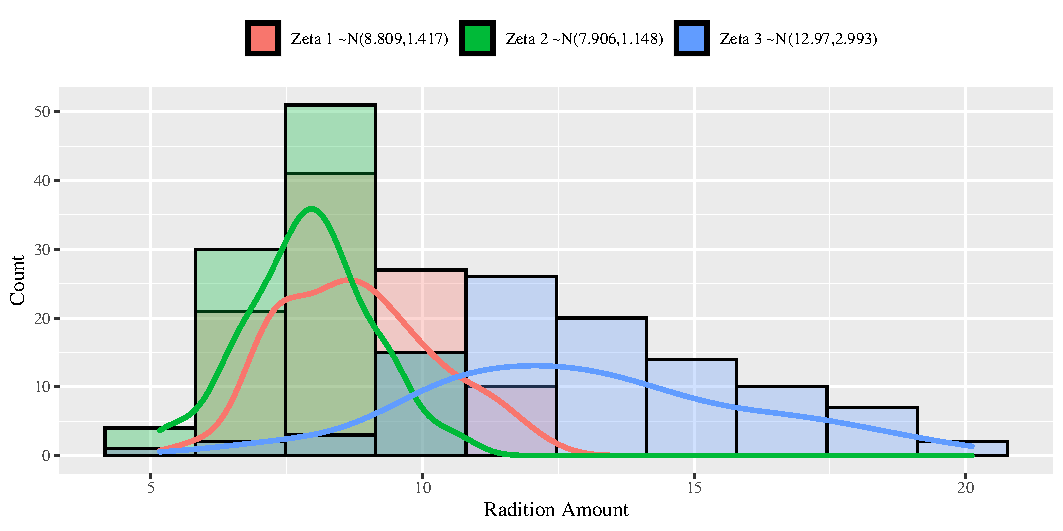
\includegraphics[width=14cm, height=7cm]{gg.zetall.pdf}
  \caption{Distribution of beam 3 radiation on normal region for random variable $\zeta_1,\zeta_2,\zeta_3$. The smooth line is a dimensionless expression of the random variables spread (density plot) whereas the histogram illustrates the number of occurrences per bin.}
  \label{fig:q2a.zeta}
\end{figure}

\begin{figure}[!tbp]
  \centering
  \subfloat[Distribution of random variable $\eta_1$.]{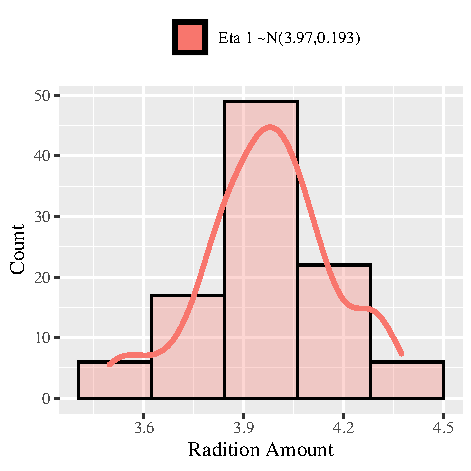
\includegraphics[width=7cm, height =7cm]{gg.eta1.pdf}\label{fig:eta1}}
  \hfill
    \subfloat[Distribution of random variable $\eta_2,\eta_3$.]{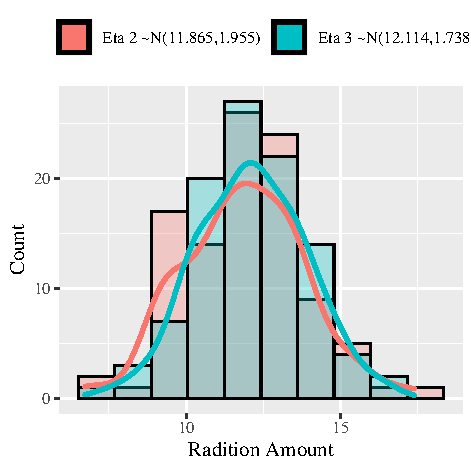
\includegraphics[width=7cm, height =7cm]{gg.eta23.pdf}\label{fig:eta23}}
  \caption{Distribution of beam 4 radiation on normal region for random variable $\eta_1,\eta_2,\eta_3$. The smooth line is a dimensionless expression of the random variables spread (density plot) whereas the histogram illustrates the number of occurrences per bin. These plots where expressed separately as the magnitude of the counts differed greatly.}
  \label{fig:q2a.eta}
\end{figure}


\newpage 
%================================================

\section{Question 2 b}

\subsection{Model formulation}

\begin{tabular}{ll}
$S^n$ & set of normal regions $S^n \in (1,2,3)$ \\
$S^t$ & set of tumour regions $S^t \in (1,2,3)$ \\
$I$ & set of beams $I \in (1,\dots, 6)$ 
\end{tabular}\\

\vspace{12pt}

\begin{tabular}{ll}
$x_{is^n}\triangleq$ & $\begin{cases}
                    1 & \text{if beam $i$ is used on region $s^n$, where $i\in I$,$s^n \in S^n$} \\
                    0 & \text{otherwise}
                    \end{cases}$ \\\\
$y_i\triangleq$ & $\begin{cases}
                    1 & \text{if beam $i$ is used, where $i\in I$} \\
                    0 & \text{otherwise}
                    \end{cases}$ \\\\
$r_{is^n} \triangleq$ & radiation from beam $i$ hitting normal region $s^n$, where $s^n \in S^n$\\
$r_{is^t} \triangleq$ & radiation from beam $i$ hitting tumour region $s^t$, where $s^t \in S^t$\\
\end{tabular}

\vspace{12pt}

The objective function maximises radiation hitting tumour regions $r_{s^t}$. 

\begin{equation}
	\max z = \sum_{i\in I}\sum_{s^t \in S^t} x_{is^t}r_{is^t}
\end{equation}

The fifth and fourth beams are denoted as random variables such that $\tilde{r}_{3s^n} = \{\tilde{\zeta}_1,\tilde{\zeta}_2,\tilde{\zeta}_3\}$ and $\tilde{r}_{4s^n} = \{\tilde{\eta}_1,\tilde{\eta}_2,\tilde{\eta}_3\}$. A deterministic equivalent is formulated using the expected value of the random variables. These values are estimated using the mean from the provided samples resulting in the following estimated parameters. 

\begin{align}
	\tilde{r}_{3s^n} = \{8.809,7.906,12.97\} \\
	\tilde{r}_{4s^n} = \{3.97,11.865,12.114 \} 
\end{align}


Subject to

\begin{align}
\label{q2b:con1}
	\sum_{i =\{1,2,5,6\}}x_{i1}r_{i1} +x_{31}E(\tilde{\zeta}_1)+ x_{41}E(\tilde{\eta}_1)\leq 40 && \\
\label{q2b:con2}
	\sum_{i =\{1,2,5,6\}}x_{i2}r_{i2} +x_{32}E(\tilde{\zeta}_2)+ x_{42}E(\tilde{\eta}_2)\leq 40 && \\
\label{q2b:con3}
	\sum_{i =\{1,2,5,6\}}x_{i3}r_{i3} +x_{33}E(\tilde{\zeta}_3)+ x_{43}E(\tilde{\eta}_3)\leq 40 && \\
\label{q2b:con4}
	\sum_{s^n \in S^n}x_{is^n}=3y_i &&  \forall i \in I \\
\label{q2b:con5}
	 x_{is^n},y_i \geq 0 && \forall i \in I, \forall s^n \in S^n
\end{align}

Constraint \ref{q2a:con1},\ref{q2a:con2} and \ref{q2a:con3} ensure that the radiation hitting a normal region is below the hazardous threshold, estimated as $E(\tilde{\eta})=\{8.81,  7.91, 12.97\}$ and $E(\tilde{\zeta}=\{3.97, 11.86, 12.11\})$. Constraint \ref{q2a:con4} ensures that if a beam is used on one region, it shall remain active for all other regions. Constraint \ref{q2a:con5} is the non-negativity constraint.

\subsection{Results}

Using \texttt{R} and the \texttt{LpSolve} package, the code snippet \ref{code:q1c} yields the resulting solution.
\begin{align}
\max z = 151 \\
x_{is^n}=
	\begin{bmatrix}
    0   & 0  &  0 \\
    1   & 1  &  1 \\
    1   & 1 &   1 \\
    1   & 1 &   1 \\
    0   & 0   & 0 \\ 
    1  &  1  &  1 \\
\end{bmatrix}
\end{align}

Beams 2,3,4 and 6 are to be used to maximise the objective function. The radiation hitting each normal region is $r_{s^n}=\{32.78, 36.77, 38.08\}$ respectively, and the radiation hitting each tumour region is $r_{s^t}=\{47, 53, 51\}$ repectively. If a beam is used on one region it is used on all regions, as per constraint, thus all constraints are adhered to. 

\subsection{Code snippets}
\label{q2a:Code}
\begin{verbatim}
	#solve expected value model

library(tidyverse)
library(lpSolve)

matMaker <- function(ones,len){
  temp <- rep(0,len)
  temp[ones] <- 1
  return(temp)
}

matMaker(c(1,2,3),100)

data.meanRadition <- read.csv(file = "RadiationData.csv", sep = ";") 
							%>% summarise_all("mean")
 							%>% as.numeric()
#                   N  N  N  T  T T
data.Radiation <- c(16,12,8,20,12,6,
                    12,10,6,18,15,8,
                    data.meanRadition[1:3],13,10,17,
                    data.meanRadition[4:6],6,18,16,
                    9,4,11,13,5,14,
                    8,7,7,10,10,10)

data.Radiation.Normal <- c(16,12,8,
                           12,10,6,
                           data.meanRadition[1:3],
                           data.meanRadition[4:6],
                           9,4,11,
                           8,7,7)

data.Radiation.tumour <- c(20,12,6,
                           18,15,8,
                           13,10,17,
                           6,18,16,
                           13,5,14,
                           10,10,10)

# Define lpsolve parameters


obj <- c(data.Radiation.tumour,rep(0,6))

constraint1.value <- c(matMaker(c(1,4,7,10,13,16),18)*data.Radiation.Normal,rep(0,6))
constraint2.value <- c(matMaker(c(2,5,8,11,14,17),18)*data.Radiation.Normal,rep(0,6))
constraint3.value <- c(matMaker(c(3,6,9,12,15,18),18)*data.Radiation.Normal,rep(0,6))

constraint4.value <- matrix(c(matMaker(c(1:3,19),24)+matMaker(19,24)*-4,
                              matMaker(c(4:6,20),24)+matMaker(20,24)*-4,
                              matMaker(c(7:9,21),24)+matMaker(21,24)*-4,
                              matMaker(c(10:12,22),24)+matMaker(22,24)*-4,
                              matMaker(c(13:15,23),24)+matMaker(23,24)*-4,
                              matMaker(c(16:18,24),24)+matMaker(24,24)*-4),
                              ncol = 24,byrow = T)

constraint.dir <- c(rep("<=",3),
                    rep("=",6))
constraint.rhs <- c(rep(40,3),
                    rep(0,6))

q2b.lp <- lp(direction = "max",
   objective.in = obj,
   const.mat = rbind(constraint1.value,
   					constraint2.value,
   					constraint3.value,
   					constraint4.value),
   const.dir = constraint.dir,
   const.rhs = constraint.rhs,
   all.bin = T)

q2b.lp
beams <- q2b.lp$solution[1:18] %>% matrix(ncol = 3,byrow = T)
q2b.lp$solution[19:24] %>% matrix(nrow = 6,byrow = T)

as.matrix(beams *matrix(data.Radiation.Normal,ncol = 3,byrow = T))%>%
						 colSums() %>% 
						 round(digits = 2)
as.matrix(beams *matrix(data.Radiation.tumour,ncol = 3,byrow = T))%>% colSums()


\end{verbatim}

\newpage
%================================================

\section{Question 2 c}

\subsection{Model formulation}

\begin{tabular}{ll}
$S^n$ & set of normal regions $S^n \in (1,2,3)$ \\
$S^t$ & set of tumour regions $S^t \in (1,2,3)$ \\
$I$ & set of beams $I \in (1,\dots, 6)$ 
\end{tabular}\\

\vspace{12pt}

\begin{tabular}{ll}
$x_{is^n}\triangleq$ & $\begin{cases}
                    1 & \text{if beam $i$ is used on region $s^n$, where $i\in I$,$s^n \in S^n$} \\
                    0 & \text{otherwise}
                    \end{cases}$ \\\\
$y_i\triangleq$ & $\begin{cases}
                    1 & \text{if beam $i$ is used, where $i\in I$} \\
                    0 & \text{otherwise}
                    \end{cases}$ \\\\
$r_{is^n} \triangleq$ & radiation from beam $i$ hitting normal region $s^n$, where $s^n \in S^n$\\
$r_{is^t} \triangleq$ & radiation from beam $i$ hitting tumour region $s^t$, where $s^t \in S^t$\\
\end{tabular}


\vspace{12pt}

The fifth and fourth beams are denoted as random variables such that $\tilde{r}_{3s^n} = \{\tilde{\zeta}_1,\tilde{\zeta}_2,\tilde{\zeta}_3\}$ and $\tilde{r}_{4s^n} = \{\tilde{\eta}_1,\tilde{\eta}_2,\tilde{\eta}_3\}$. A deterministic equivalent can be formulated using chance constraint programming and the scenario approach by generating $N$ scenarios sampled from each random variable to ensure a set of $N$ constraints are satisfied 99\% of the time.

The constraints containing random variables are expressed as

\begin{align}
	P\bigg{(}\sum_{i =\{1,2,5,6\}}x_{i1}r_{i1} +x_{3}\tilde{\zeta}_1+ x_{4}\tilde{\eta}_1\leq 40 \bigg{)} \geq 1-0.01&& \\
	P\bigg{(}\sum_{i =\{1,2,5,6\}}x_{i2}r_{i2} +x_{3}\tilde{\zeta}_2+ x_{4}\tilde{\eta}_2\leq 40 \bigg{)} \geq 1-0.01&& \\
	P\bigg{(}\sum_{i =\{1,2,5,6\}}x_{i3}r_{i3} +x_{3}\tilde{\zeta}_3+ x_{4}\tilde{\eta}_3\leq 40 \bigg{)} \geq 1-0.01&&
\end{align}

where $P$ is the probability of the constraint being satisfied 99\% of the time. The percentage is expressed as $1-0.01 = 0.99$ such that $\alpha = 0.01$. There are 2 random variables per constraint resulting in $n=2$. A 99\% confidence interval is selected, setting $\delta = 0.01$. The confidence interval ensures that the sample $N$ is large enough for the constraint to be adhered to. $N$ is calculated as follows.

\begin{align}
	N=&[ 2n\alpha^{-1}\ln(\frac{12}{\alpha}) + 2\alpha^{-1}\ln(\frac{2}{\delta})+2n] \\
	N=&[ 2(2)(0.01)^{-1}\ln(\frac{12}{(0.01)}) + 2(0.01)^{-1}\ln(\frac{2}{(0.01)})+2(2)]\\
	N=&3899.694\approx3900
\end{align}

This implies  \{$\zeta_1^q,\eta_1^q\}$, $\{\zeta_2^q,\eta_2^q\}$ and $\{\zeta_3^q,\eta_3^q\}$ will be sampled for $q\in N$ instances to generated $N$ constraints. The deterministic formulation is defines as follows.

\begin{equation}
	\max z = \sum_{i\in I}\sum_{s^t \in S^t} x_{is^t}r_{is^t}
\end{equation}

Subject to

\begin{align}
\label{q2c:cons1}
	\sum_{i =\{1,2,5,6\}}x_{i1}r_{i1} +x_{31}\zeta_1^q+ x_{41}\eta_1^q\leq 40 && \forall q \in N\\
\label{q2c:cons2}
	\sum_{i =\{1,2,5,6\}}x_{i2}r_{i2} +x_{32}\zeta_2^q+ x_{42}\eta_2^q\leq 40 && \forall q \in N\\
\label{q2c:cons3}
	\sum_{i =\{1,2,5,6\}}x_{i3}r_{i3} +x_{33}\zeta_3^q+ x_{43}\eta_3^q\leq 40 && \forall q \in N\\
\label{q2c:cons4}
	\sum_{s^n \in S^n}x_{is^n}=3y_i &&  \forall i \in I \\
\label{q2c:cons5}
	 y_i \geq 0 && \forall i \in I\\
\label{q2c:cons6}
	 x_{is^n} \geq 0 && \forall i \in I,\forall s^n \in S^n 
\end{align}

Constraints \ref{q2c:cons1}, \ref{q2c:cons2} and \ref{q2c:cons3} ensure that the radiation hitting a normal region is below the hazardous threshold, estimated by generating $N=3900$ constraints. Thus these constraints are a condensed expression of all possible constraints. The constraint values are sampled from a distribution to ensure a 99\% confidence interval. The remaining constraints are defined as in the previous section.

\subsection{Results}

To implement the solution, a 18 by 3904 matrix was formulated in which columns 7 to 12 denote the random variables. Each row in columns 7 to 12 is a value sampled from a normal distribution using the \texttt{rnorm()} function. The input parameters are the respective means and standard deviations of the random variables. Using \texttt{R} and the \texttt{LpSolve} package, the code snippet \ref{code:q2c} yields the resulting solution.
\begin{align}
\max z = 41 \\
x_{is^n}=
	\begin{bmatrix}
    0  &  0  &  0 \\
    1  &  1  &  1 \\
    0  &  0  &  0 \\ 
    0  &  0  &  0 \\
    0  &  0  &  0 \\
    0  &  0  &  0
\end{bmatrix}
\end{align}

Only beam 2 is be used to maximise the objective function when compared to the expected value approach which activated beams 2,3,4 and 6. The radiation hitting the each tumour region is $r_{s^t}=\{18 ,15,  8\}$ respectively. The result is far lower than the expected value approach, indicating a far more restricting constraint. This approximation is more conservative yet yields a lower objective function and $r_{s^t}$. No constraint are violated.


\label{code:q2c}
\subsection{Code snippets}

\begin{verbatim}
	#solve approximation model

library(tidyverse)
library(lpSolve)

matMaker <- function(ones,len){
  temp <- rep(0,len)
  temp[ones] <- 1
  return(temp)
}

data.meanRadition <- read.csv(file = "RadiationData.csv", sep = ";") 
%>% summarise_all("mean") 
%>% as.numeric()
data.sdRadition <- read.csv(file = "RadiationData.csv", sep = ";") 
%>% summarise_all("sd") 
%>% as.numeric()

N = 3900


data.Radiation.Normal <- c(16,12,8,
                           12,10,6,
                           0,0,0,
                           0,0,0,
                           9,4,11,
                           8,7,7)

data.Radiation.tumour <- c(20,12,6,
                           18,15,8,
                           13,10,17,
                           6,18,16,
                           13,5,14,
                           10,10,10)

constraint1.value <- rep(data.Radiation.Normal,N) %>% matrix(ncol = 18,byrow = T)

for (i in 7:12){
  constraint1.value[,i] <- round(rnorm(n = N,
  									 mean =data.meanRadition[i-6] ,
  									 sd = data.sdRadition[i-6]),
  									 digits = 4)
}
constraint1.value <- cbind(constraint1.value,matrix(data = 0,nrow = N,ncol = 6))

# Define lpsolve parameters


obj <- c(data.Radiation.tumour,rep(0,6))

constraint2.value <- matrix(c(matMaker(c(1:3,19),24)+matMaker(19,24)*-4,
                              matMaker(c(4:6,20),24)+matMaker(20,24)*-4,
                              matMaker(c(7:9,21),24)+matMaker(21,24)*-4,
                              matMaker(c(10:12,22),24)+matMaker(22,24)*-4,
                              matMaker(c(13:15,23),24)+matMaker(23,24)*-4,
                              matMaker(c(16:18,24),24)+matMaker(24,24)*-4),
                              ncol = 24,byrow = T)

constraint.dir <- c(rep("<=",N),
                    rep("=",6))
constraint.rhs <- c(rep(40,N),
                    rep(0,6))

q2c.lp <- lp(direction = "max",
             objective.in = obj,
             const.mat = rbind(constraint1.value,constraint2.value),
             const.dir = constraint.dir,
             const.rhs = constraint.rhs,
             all.bin = T)

q2c.lp
beams <- q2b.lp$solution[1:18] %>% matrix(ncol = 3,byrow = T)
q2b.lp$solution[19:24] %>% matrix(nrow = 6,byrow = T)
beams




\end{verbatim}


\newpage
%================================================

\section{Question 2 d}
\subsection{Model formulation}
\begin{tabular}{ll}
$S^n$ & set of normal regions $S^n \in (1,2,3)$ \\
$S^t$ & set of tumour regions $S^t \in (1,2,3)$ \\
$I$ & set of beams $I \in (1,\dots, 6)$ 
\end{tabular}\\

\vspace{12pt}

\begin{tabular}{ll}
$x_{is^n}\triangleq$ & $\begin{cases}
                    1 & \text{if beam $i$ is used on region $s^n$, where $i\in I$,$s^n \in S^n$} \\
                    0 & \text{otherwise}
                    \end{cases}$ \\\\
$y_i\triangleq$ & $\begin{cases}
                    1 & \text{if beam $i$ is used, where $i\in I$} \\
                    0 & \text{otherwise}
                    \end{cases}$ \\\\
$r_{is^n} \triangleq$ & radiation from beam $i$ hitting normal region $s^n$, where $s^n \in S^n$\\
$r_{is^t} \triangleq$ & radiation from beam $i$ hitting tumour region $s^t$, where $s^t \in S^t$\\
\end{tabular}



\vspace{12pt}

The fifth and fourth beams are denoted as random variables such that $\tilde{r}_{3s^n} = \{\tilde{\zeta}_1,\tilde{\zeta}_2,\tilde{\zeta}_3\}$ and $x_4\tilde{r}_{4s^n} = \{\tilde{\eta}_1,\tilde{\eta}_2,\tilde{\eta}_3\}$. Figure~\ref{fig:q2a.zeta} and Figure~\ref{fig:q2a.eta} provide justification to assume that the random variables are rotationally invariant (symmetrical distributions) thus permitting the use of chance constraint approximation methods. The constraints may be modelled as follows.
\begin{align}
\label{eq:2d48}
	P\bigg{(}\sum_{i =\{1,2,5,6\}}x_{i1}r_{i1} +x_{3}\tilde{\zeta}_1+ x_{4}\tilde{\eta}_1\leq 40 \bigg{)} \geq 1-0.01&& \\
\label{eq:2d49}
	P\bigg{(}\sum_{i =\{1,2,5,6\}}x_{i2}r_{i2} +x_{3}\tilde{\zeta}_2+ x_{4}\tilde{\eta}_2\leq 40 \bigg{)} \geq 1-0.01&& \\
\label{eq:2d50}
	P\bigg{(}\sum_{i =\{1,2,5,6\}}x_{i3}r_{i3} +x_{3}\tilde{\zeta}_3+ x_{4}\tilde{\eta}_3\leq 40 \bigg{)} \geq 1-0.01&&
\end{align}


There are two random variables per constraint resulting in $m=2$ and $\alpha = 0.01$ which allows $\Omega$ to be calculated as follows.
\begin{align}
	\Omega &= \bigg{(} \sqrt{2 \ln \frac{2}{0.01}} \bigg{)}  \\
			&=3.255247 \approx 3.255
\end{align}


Using $\Omega$ and converting the equations in the approximation method's standard form,  It should be noted that $x_i$ is a binary variable and as such there is no impact of raising $x_i$ to any power. This property assists in reducing equation~\ref{eq:2d48} as follows.

\begin{align}
\sum_{i =\{1,2,5,6\}}x_{i1}r_{i1} -40+x_{31}(\bar{\zeta}_1+\tilde{\zeta}_1^\prime)+ x_{41}(\bar{\eta}_1+\tilde{\eta}_1^\prime)\leq 0 && \\
\bigg{[}\sum_{i =\{1,2,5,6\}}x_{i1}r_{i1} + x_{31}\bar{\zeta}_1+ x_{41}\bar{\eta}_1 -40\bigg{]} +\Omega \big{(}(x_{31}((\tilde{\zeta}_1^\prime)^2\times 1^2)^\frac{1}{2} +x_{41}((\tilde{\eta}_1^\prime)^2\times 1^2)^\frac{1}{2}\big{)}\leq 0 && \\ %line 2
\bigg{[}\sum_{i =\{1,2,5,6\}}x_{i1}r_{i1} + 8.809x_{31}+ 3.970x_{41} -40\bigg{]} +3.255 \big{(}1.417x_{31} + 0.193x_{41}\big{)}\leq 0 && \\ %line 3
\sum_{i =\{1,2,5,6\}}x_{i1}r_{i1} + 13.421x_{31} + 4.598x_{41} \leq 40 && %line 4
\end{align}

The random variables are approximated as $\tilde{\zeta}_1 \approx 13.421$ and $\tilde{\eta}_1 \approx 4.598$. Equation~\ref{eq:2d49} and Equation~\ref{eq:2d50} were reduced using the same method, resulting in $\tilde{\zeta}_2 \approx 11.644$, $\tilde{\eta}_2 \approx 18.230$, $\tilde{\zeta}_3 \approx 22.714$ and $\tilde{\eta}_3 \approx 17.772$. Leading to the following deterministic formulation.


\begin{table}[]
\caption{Fixed and variable components used in the approximation approach.}
\label{tbl:q2d}
\vspace{12pt}
\centering
\begin{tabular}{ccccccc}
\hline
$s^n$ & $\bar{\zeta}_{s^n}$ & $\tilde{\zeta}_{s^n}^\prime$ & $\bar{\eta}_{s^n}$ & $\tilde{\eta}_{s^n}^\prime$ & $\zeta^{\prime2}_{s^n}$ & $\eta^{\prime2}_{s^n}$\\
\hline
1           & 8.809             & N(0,1.417)      & 3.970      & N(0,0.193) & 2.008 &0.037\\
2           & 7.906             & N(0,1.148)      & 11.865     & N(0,1.955) & 1.319 &3.824\\
3           & 12.97             & N(0,2.993)      & 12.114     & N(0,1.738) & 8.959&3.021\\
 
\hline
\end{tabular}
\end{table}




\begin{equation}
	\max z = \sum_{i\in I}\sum_{s^t \in S^t} x_{is^t}r_{is^t}
\end{equation}

Subject to

\begin{align}
\label{q2e:cons1}
	\sum_{i =\{1,2,5,6\}}x_{i1}r_{i1} + 13.421x_{31} + 4.598x_{41} \leq 40 && \\%line 1
\label{q2e:cons2}
	\sum_{i =\{1,2,5,6\}}x_{i1}r_{i1} + 11.644x_{32} + 18.230x_{42} \leq 40 &&\\ %line 2
\label{q2e:cons3}
	\sum_{i =\{1,2,5,6\}}x_{i1}r_{i1} + 22.714x_{33} + 17.772x_{43} \leq 40 &&\\ %line 3
\label{q2e:cons4}
	\sum_{s^n \in S^n}x_{is^n}=3y_i &&  \forall i \in I \\
\label{q2e:cons5}
	 y_i \geq 0 && \forall i \in I\\
\label{q2e:cons6}
	 x_{is^n} \geq 0 && \forall i \in I,\forall s^n \in S^n 
\end{align}


Constraints \ref{q2e:cons1}, \ref{q2e:cons2} and \ref{q2e:cons3} ensure that the radiation hitting a normal region is below the hazardous threshold, estimated using the analytical approximation approach. The remaining constraints are defined as in the previous section.


\subsection{Results}

To implement the solution, a 18 by 3904 matrix was formulated in which columns 7 to 12 denote the random variables. Each row in columns 7 to 12 is a value sampled from a normal distribution using the \texttt{rnorm()} function. The input parameters are the respective means and standard deviations of the random variables. Using \texttt{R} and the \texttt{LpSolve} package, the code snippet \ref{code:q2c} yields the resulting solution.
\begin{align}
\max z = 113 \\
x_{is^n}=
	\begin{bmatrix}
    0  &  0  &  0 \\
    1  &  1  &  1 \\
    0  &  0  &  0 \\
    1  &  1  &  1 \\
    1  &  1  &  1 \\
    0  &  0   & 0 \\
\end{bmatrix}
\end{align}

Using the scenario approach resulted in only beam 2 being selected whereas the analytical approximation includes beam 4 and 5. Compared to the expected value approach, one less beam is used and beam 5 is activated instead of beam 6 resulting in a marginally lower object function value. The radiation hitting each tumour region is $r_{s^t}=\{37, 38, 38\}$ respectively and the radiation hitting each normal region is $r_{s^t}=\{25.60 ,32.23, 34.77\}$ respectively. This approximation slightly more conservative than the expected value approach yet far more lenient than the scenario approach. No constraints are violated.

\newpage
%================================================

\section{Question 2 e}
\subsection{Model formulation}
\begin{tabular}{ll}
$x_i\triangleq$ & $\begin{cases}
                    1 & \text{if beam $i$ is used , where $i\in I$ and $I= \{1,\ldots,6\} $} \\
                    0 & \text{otherwise}
                    \end{cases}$ \\\\
$r_{is^n} \triangleq$ & radiation from beam $i$ hitting normal region $s^n$, where $s^n \in S^n$ and $S^n=\{1,2,3\}$\\
$r_{is^t} \triangleq$ & radiation from beam $i$ hitting tumour region $s^t$, where $s^t \in S^t$ and $S^n=\{1,2,3\}$\\
\end{tabular}

\vspace{12pt}

The fifth and fourth beams are denoted as random variables such that $\tilde{r}_{3s^n} = \{\tilde{\zeta}_1,\tilde{\zeta}_2,\tilde{\zeta}_3\}$ and $x_4\tilde{r}_{4s^n} = \{\tilde{\eta}_1,\tilde{\eta}_2,\tilde{\eta}_3\}$. Two additional variables are introduced to initiate the recourse model formulation.
\vspace{12pt}

\begin{tabular}{ll}
$\delta_{s^n}^- \triangleq$ & excess levels of radiation hitting normal region $s^n$, where $s^n \in S^n$.\\
$\delta_{s^n}^+ \triangleq$ & reduced levels of radiation hitting normal region $s^n$, where $s^n \in S^n$.\\\\
\end{tabular}

\begin{equation}
	\max z = \sum_{i\in I}\sum_{s^t \in S^t} x_ir_{is^t} -\sum_{s^n \in S^n}E_{\tilde{\zeta},\tilde{\eta}}\big{(}2\delta_{s^n}^-(\tilde{\zeta}, \tilde{\eta})\big{)}
\end{equation}

Subject to

\begin{align}
	\sum_{i =\{1,2,5,6\}}x_ir_{i1} +x_{3}\tilde{\zeta}_1+ x_{4}\tilde{\eta}_1+\delta_1^+(\tilde{\zeta}, \tilde{\eta})-\delta_1^-(\tilde{\zeta}, \tilde{\eta})= 40 && \\
	\sum_{i =\{1,2,5,6\}}x_ir_{i2} +x_{3}\tilde{\zeta}_2+ x_{4}\tilde{\eta}_2+\delta_2^+(\tilde{\zeta}, \tilde{\eta})-\delta_2^-(\tilde{\zeta}, \tilde{\eta}) = 40 && \\
	\sum_{i =\{1,2,5,6\}}x_ir_{i3} +x_{3}\tilde{\zeta}_3+ x_{4}\tilde{\eta}_3+\delta_3^+(\tilde{\zeta}, \tilde{\eta})-\delta_3^-(\tilde{\zeta}, \tilde{\eta}) = 40 && \\
	 x_i \geq 0 && \forall i \in I \\
	 \delta_{s^n}^-,\delta_{s^n}^+ \geq 0 && \forall s^n \in S^n
\end{align}


Discrete equivalents of the random variables must be generated. As there are two random variables in the constraints, two sets of random variables $R1=\{1,2,3\}$ and $R_2=\{1,2,3\}$ are generated. Three bins have been chosen to reduce the number of constraints in the formulation, noting that increasing the number of bins will yield a more accurate solution.


\begin{table}[]
\centering
\begin{tabular}{cccc}
\hline
\textbf{Prob} & \textbf{Impact} & \textbf{Variable} & \textbf{Bin}\\
\hline
0.0777        & 4.9644          & $\zeta_1^{r_1}$        &       1        \\
0.8061        & 8.6638          & $\zeta_1^{r_1}$         &       2       \\
0.1162        & 12.3631         & $\zeta_1^{r_1}$          &       3       \\
0.1487        & 5.2685          & $\eta_1^{r_1}$            &     1       \\
0.7802        & 8.1425          & $\eta_1^{r_1}$           &      2       \\
0.0711        & 11.0164         & $\eta_1^{r_1}$           &      3       \\
0.1319        & 5.9366          & $\zeta_2^{r_1}$          &      1        \\
0.7789        & 13.3082         & $\zeta_2^{r_1}$          &      2        \\
0.0892        & 20.6799         & $\zeta_2^{r_1}$          &      3        \\
0.0781        & 3.4631          & $\eta_2^{r_1}$           &      1       \\
0.7801        & 3.9389          & $\eta_2^{r_1}$           &      2       \\
0.1418        & 4.4147          & $\eta_2^{r_1}$           &      3       \\
0.1140        & 7.0992          & $\zeta_3^{r_1}$          &      1        \\
0.7754        & 11.9197         & $\zeta_3^{r_1}$          &      2        \\
0.1106        & 16.7401         & $\zeta_3^{r_1}$          &      3        \\
0.1065        & 7.9167          & $\eta_3^{r_1}$           &      1       \\
0.7765        & 12.1088         & $\eta_3^{r_1}$           &      2       \\
0.1170        & 16.3008         & $\eta_3^{r_1}$           & 	  3		\\
\hline                 
\end{tabular}
\caption{}
\label{tab:q2ProbSummary}
\end{table}


\begin{equation}
	\max z = \sum_{i\in I}\sum_{s^t \in S^t} x_ir_{is^t} -\sum_{r_1=1}^3\sum_{r_2=1}^3p_1^{r_1}p_2^{r_2}\big{(}2\delta_1^{-,r_1,r_2}\big{)}
\end{equation}

Subject to

\begin{align}
	\sum_{i =\{1,2,5,6\}}x_ir_{i1} +x_{3}\zeta_1^{r_1}+ x_{4}\eta_1^{r_2}+\delta_1^{+,r_1,r_2}-\delta_1^{-,r_1,r_2}= 40 && \forall r_1 \in R_1, \forall r_2 \in R_2\\
	\sum_{i =\{1,2,5,6\}}x_ir_{i2} +x_{3}\zeta_2^{r_1}+ x_{4}\eta_2^{r_2}+\delta_2^{+,r_1,r_2}-\delta_2^{-,r_1,r_2}= 40 && \forall r_1 \in R_1, \forall r_2 \in R_2\\
	\sum_{i =\{1,2,5,6\}}x_ir_{i3} +x_{3}\zeta_3^{r_1}+ x_{4}\eta_3^{r_2}+\delta_3^{+,r_1,r_2}-\delta_3^{-,r_1,r_2}= 40 && \forall r_1 \in R_1, \forall r_2 \in R_2\\
	 x_i \geq 0 && \forall i \in I \\
	 \delta_{s^n}^-,\delta_{s^n}^+ \geq 0 && \forall s^n \in S^n
\end{align}


\subsection{Code snippets}

\begin{verbatim}
	
normDiscrete <- function(mean, sd, bins){
  smpl <- rnorm(n=10000, mean=mean, sd=sd)
  hist <- hist(x = smpl, breaks = seq(min(smpl),max(smpl),(max(smpl)-min(smpl))/bins))
  Probability <- hist$counts/10000
  Impact <- hist$mid
  solution <- data.frame(Probability,Impact)
  return(solution)
}


radiation.data <- read.csv(file = "RadiationData.csv", sep = ";")

data.prob <- data.frame()
# Calculating the probability and impact for zeta
for (i in 1:6){
  temp <- normDiscrete(mean = as.numeric((summarise_all(radiation.data,"mean"))[i]),
                      sd = as.numeric((summarise_all(radiation.data,"sd"))[i]), 
                      bins = 3)
  data.prob <- rbind(data.prob,
              cbind(temp,Var=names((summarise_all(radiation.data,"mean"))[i])))
}


\end{verbatim}

\newpage
%================================================

\section{Question 2 f}
\subsection{Model formulation}

\begin{tabular}{ll}
$x_i\triangleq$ & $\begin{cases}
                    1 & \text{if beam $i$ is used , where $i\in I$ and $I= \{1,\ldots,6\} $} \\
                    0 & \text{otherwise}
                    \end{cases}$ \\\\
$r_{is^n} \triangleq$ & radiation from beam $i$ hitting normal region $s^n$, where $s^n \in S^n$ and $S^n=\{1,2,3\}$\\
$r_{is^t} \triangleq$ & radiation from beam $i$ hitting tumour region $s^t$, where $s^t \in S^t$ and $S^n=\{1,2,3\}$\\
\end{tabular}

\vspace{12pt}

\begin{tabular}{ll}
$\delta_{s^n}^- \triangleq$ & excess levels of radiation hitting normal region $s^n$, where $s^n \in S^n$.\\
$\delta_{s^n}^+ \triangleq$ & reduced levels of radiation hitting normal region $s^n$, where $s^n \in S^n$.\\\\
\end{tabular}

The fifth and fourth beams are denoted as random variables such that $\tilde{r}_{3s^n} = \{\tilde{\zeta}_1,\tilde{\zeta}_2,\tilde{\zeta}_3\}$ and $x_4\tilde{r}_{4s^n} = \{\tilde{\eta}_1,\tilde{\eta}_2,\tilde{\eta}_3\}$. In addition to the variables included in the recourse approach, a new variable is introduce to determine the reliability of the model.
\vspace{12pt}

\begin{tabular}{ll}
$r_n\triangleq$ & $\begin{cases}
                    1 & \text{if either $z^\text{actual}\leq z^\star$, or $\delta_{s^n}^-+\delta^+_{s^n}=0$} \\
                    0 & \text{otherwise}
                    \end{cases}$ \\\\
\end{tabular}

\vspace{12pt}

The reliability may then be calculated as

\begin{equation}
	\frac{1}{N}	\sum_{n\in \{1,\dots,N\}} r_n
\end{equation}

A quick comparison between the expected value approach and the analytical approximation approach reveals that the expected value approach obtained a smaller difference between the maximum radiation levels for normal tissue, leading it to be less conservative. By deduction, the scenario approach is the most constraining and thus caters for greater spread of possibilities.

\end{document}
